\subsection{Opgaver}

 \begin{enumerate}
\item 	Opskriv en andengradsligning på formen $x^2+bx+c=0$ med rødderne
\begin{align*}
2 \textup{ og } -1,&& \frac{1}{2} \textup{ og } 3,&&  -\sqrt{2} \textup{ og } \sqrt{2},&& \frac{1+\sqrt{5}}{2} \textup{ og } \frac{1-\sqrt{5}}{2}.
\end{align*}

\item Løs ligningerne
\begin{align*}
x^2=36,&&(x-1)(x+2)=0,&& 2x^2+3x+1=0,&& x^2+4x+3=0.
\end{align*}

\item Løs ligningssystemet
\begin{alignat*}{4}
x& {}+{}&y & {}={}& 4\\
\frac{1}{2}x& {}+{}&1&{}={}& 9& {}-{}&2y
\end{alignat*}

\item Løs ligningerne
\begin{align*}
2x^2-3x=0,&& 3x^2-21x=0,&& 5x^2=2x,&& \frac{(11x)^2}{49}= 1.
\end{align*}

\item Løs ligningssystemet 
\begin{alignat*}{3}
2y&{}-{}&x&{}={}&3\\
4y&{}-{}&5x&{}={}&-3
\end{alignat*}

\item Forkort følgende brøker
\begin{align*}
\frac{x^2-36}{x^2-5x-6},&& \frac{(x+1)(x^2-4x+3)}{x^2-2x-3},&&\frac{x^2-1}{x^2-3x+2}.
\end{align*}


\item Løs ligningerne
\begin{align*}
-\frac{1}{2}x^2- \frac{3}{2}x=-2,&& -2x^2+6x=-8,&& \frac{5}{2}x^2 -7x+1=0,&& 4x^2=100.
\end{align*}



\item Hvor skal man bøje en $\frac{7}{10} m$ lang stang i en ret vinkel for at afstanden mellem endepunkterne bliver:
\begin{enumerate}
\item $\frac{1}{2} m$,
\item $\frac{3}{5} m$.
\end{enumerate}

\item Løs ligningessystemet
\begin{alignat*}{5}
x&{}-{}&2y&{}+{}&5z&{}={}&24\\
-x&{}+{}&3y&{}-{}&3z&{}={}&-6\\
&{}-{}&y&{}-{}& z&{}={}&-12
\end{alignat*}


\item Løs ligningerne 
\begin{align*}
x+7-\frac{5}{x-2}=5, && \frac{3}{8}+\frac{1}{x}=-\frac{1}{2x^2},&& -\frac{1}{12x}+3x=0.
\end{align*}

\item Løs ligningerne
\begin{align*}
 \frac{4}{x^2}+\frac{16}{x-3}=0,&& x=3+\frac{70}{x},&& \frac{1}{x}- \frac{3}{x^2}=0.
\end{align*}

\item For hvilke $b$ har ligningen
\begin{align*}
2x^2+bx+2=0,
\end{align*}
præcis en løsning?

\item For hvilke $a$ har ligningen 
\begin{align*}
ax^2-4x+1=0
\end{align*}
ingen reelle løsninger?

\item Bestem de reelle løsninger til ligningerne
\begin{align*}
x^4-x^2-12=0,&& x^4=18+7x^2,&& x^6-7x^3-8=0.
\end{align*}
(Hint: Lad $y=x^2$ i de to første ligninger og $y=x^3$ i den sidste.)


\item \label{it:2poly} På Figur~\ref{fig:2poly} ses graferne for andengradspolynomierne $\frac{1}{8}x^2-\frac{1}{2}x+\frac{11}{8}$ og $-\frac{3}{4}x^2+\frac{5}{4}x+4$. Bestem polynomiernes skæringspunkter. 
\begin{figure}
\centering
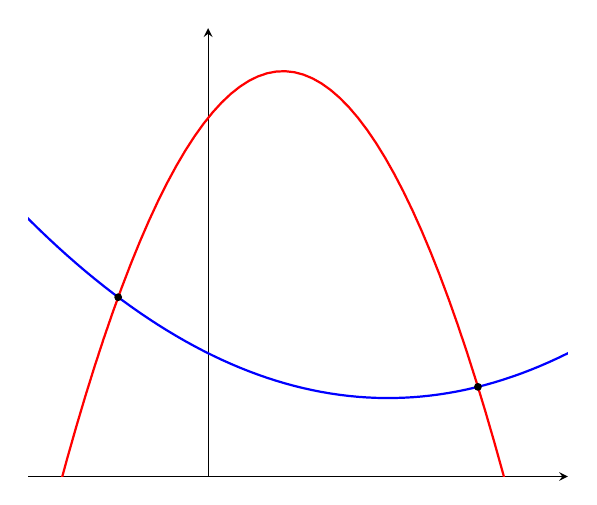
\begin{tikzpicture}
\begin{axis}[xmin=-2,xmax=4,ymin=0,ymax=5,axis x line=center,
  axis y line=center, ticks=none]
\addplot[thick,blue,samples =100] {1/8*x*x-1/2*x+11/8};
\addplot[thick,red,samples=100] {-3/4*x*x+5/4*x+4};
\node[fill, circle, inner sep=1pt] at (axis cs:-1,2) {};
\node[fill, circle, inner sep=1pt] at (axis cs:3,1) {};
\end{axis}
\end{tikzpicture}
\caption{Opgave~\ref{it:2poly}}
\label{fig:2poly}
\end{figure}

\item Løs ligningssystemet nedenfor både vha. substitution og lige store koefficienters metode.

\begin{alignat*}{5}
x & {}+{} &  y & {}+{} & z &{}+{}&w & {}={} & 34 \\
-x & {}+{} &  y & {}{} & &{}{}&  & {}={} & 1 \\
&  &  -y & {}+{} & z & & & {}={} & 1 \\
&  &   &&-z &{}+{}& w & {}={} & 1 \\
\end{alignat*}

\item \label{it:phi} På Figur~\ref{fig:phi} ses et linjestykke som er opdelt således at længderne $a$ og $b$ opfylder
\begin{align*}
\frac{a}{b}=\frac{a+b}{a}.
\end{align*}
Bestem forholdet $\phi=\frac{a}{b}$. 

(Hint: gang ligningen igennem med $\phi$ og reducer til $\phi^2=\phi+1$.)

\begin{figure}
	\centering
	\begin{tikzpicture}
	\draw (0,0)-- node[above] {$b$} (3,0) -- node[above] {$a$} ({3+3*(1+sqrt(5))/2},0);
	\node[fill, inner sep =1pt,circle] at (3,0) {};
	\end{tikzpicture}
	\caption{Opgave~\ref{it:phi}}
	\label{fig:phi}
\end{figure}

\item Papir i A format er designet således at hvis et ark deles på midten, som illustreret i Figur~\ref{fig:2deglig1}, så gælder at
\begin{align*}
\frac{b}{a}=\frac{\frac{a}{2}}{b}.
\end{align*}
Hvis $A(n)$ betegner arealet af et ark An papir i $m^2$ så gælder at
\begin{align*}
A(n)= \frac{1}{2^n}.
\end{align*}
\begin{enumerate}
	\item Bestem arealet af et A4 ark.
	\item Bestem sidelængderne af et A4 ark.
	\item Vis at sidelængderne for et An ark er givet ved
	\begin{align*}
	2^{\frac{-2n-1}{4}},\quad \textup{og}\quad 2^{ \frac{-2n+1}{4}}.
	\end{align*}
\end{enumerate}

\begin{figure}
	\centering
	\begin{tikzpicture}
	\draw (0,0)-- node[left] {$b$} (0,3)-- node[above] {$a$} ({sqrt(18)},3)--({sqrt(18)},0)--cycle;
	\draw[dashed] ({sqrt(9/2)},3)--({sqrt(9/2)},0);
	\node at (({sqrt(9/2)}/2,0) [label= below: $\frac{a}{2}$] {};
	\end{tikzpicture}
	\caption{A papirformat}
	\label{fig:2deglig1}
\end{figure}

\item Vis at løsningerne til andengradsligningen
\begin{align*}
ax^{2}+bx+x=0
\end{align*}
hvor $a\neq0$, er givet ved 
\begin{align*}
x=\frac{-b\pm \sqrt{b^2-4ac}}{2a}.
\end{align*}
(Hint: Brug Opgave~\ref{it:eks21}.)
\end{enumerate}
